\documentclass[russian,utf8,12pt,emptystyle]{eskdtext}
\usepackage{color}
\usepackage{eskdtotal}
\usepackage{eskdplain}
\usepackage{graphicx}
\usepackage{fancyhdr}
\usepackage{listings}
\usepackage{ltxtable}
\usepackage{multirow}
\usepackage{setspace}
\usepackage{tabularx}
\usepackage{pdfpages}
\usepackage{cmap}
\usepackage[unicode]{hyperref}
\usepackage{appendix}
%\usepackage[english,russian]{babel}
\usepackage{underscore}
\usepackage{longtable}
\newcommand{\No}{\textnumero}
\begin{document}
\DeclareGraphicsExtensions{.png}
\graphicspath{{images/}}
\ESKDsectSkip{section}{10pt}{10pt}
\ESKDsectSkip{subsection}{8pt}{8pt}
\ESKDsectSkip{subsubsection}{8pt}{8pt}
\begin{abstract}
Документ определяет порядок демонстрации работы системы от нажатия кнопки до назначения машины для выполнения работ.
\end{abstract}
\section*{Термины и определения}
\begin{longtable}[h]{|p{0.25\linewidth}|p{0.65\linewidth}|}
\hline
\textbf{Термин}&\textbf{Определение}\\
\hline
Новарис ERP& подсистема управления предприятием\\
\hline
Новарис NCS& подсистема голосовых оповещений\\
\hline
Новарис NMS& подсистема мониторинга и навигации\\
\hline 
Платформа& система управления и контроля обработки услуг, состоящая из Новарис ERP, Новарис NCS и Новарис NMS\\
\hline
Клиент& физическое или юридическое лицо обладающее автотранспортом оборудованной системой спутникового мониторинга, запрашивающее предоставление услуги\\
\hline
Поставщик услуги& физическое или юридической лицо обладающее автотранспортом оборудованной системой спутникового мониторинга, предоставляющее запрашиваемую услугу\\
\hline
Оператор услуги& ответственный пользователь от Поставщика услуги, имеющий доступ к Платформе для управления запрошенными услугами\\
\hline
Оператор платформы& администратор системы имеющий полный доступ к управлению Платформой\\
\hline
\end{longtable}
\vspace{1cm}
\section*{Ограничения}
Ограничения на этапе первичной демонстрации (предмет дальнейшей доработки системы):
\begin{itemize}
\item поиск ведётся ближайшей свободной сервисной машины (без учёта договоров)
\item для отображения автомобилей используется пока только одна карта Google Maps
\end{itemize} 
\section{Начальное состояние}
\label{begin}
На обоих машинах установлено навигационное оборудование с контролем нажатия кнопки.

На клиентской машине датчик нажатия кнопки определён как <<Тревожная кнопка>> (тип 5)

На сервисной машине датчика нажатия кнопки определён как <<Кнопка статуса автомобиля>> (тип 6)

При этом предполагается, что нажатие кнопки сервисной машины определяет занятость и исключает её из поиска. 

Все события в БД очищены для более чёткой демонстрации работы системы.

В системе проверено поступление данных о координатах и состояние датчиков, блоки настроен на максимальную приоритезацию событий по нажатию клавиши. Задержка от нажатия кнопки до поступления данных в систему не превышает 5 сек.

Пример настройки клиентской машины:
  \begin{figure}[h]
  \begin{center}
  \center{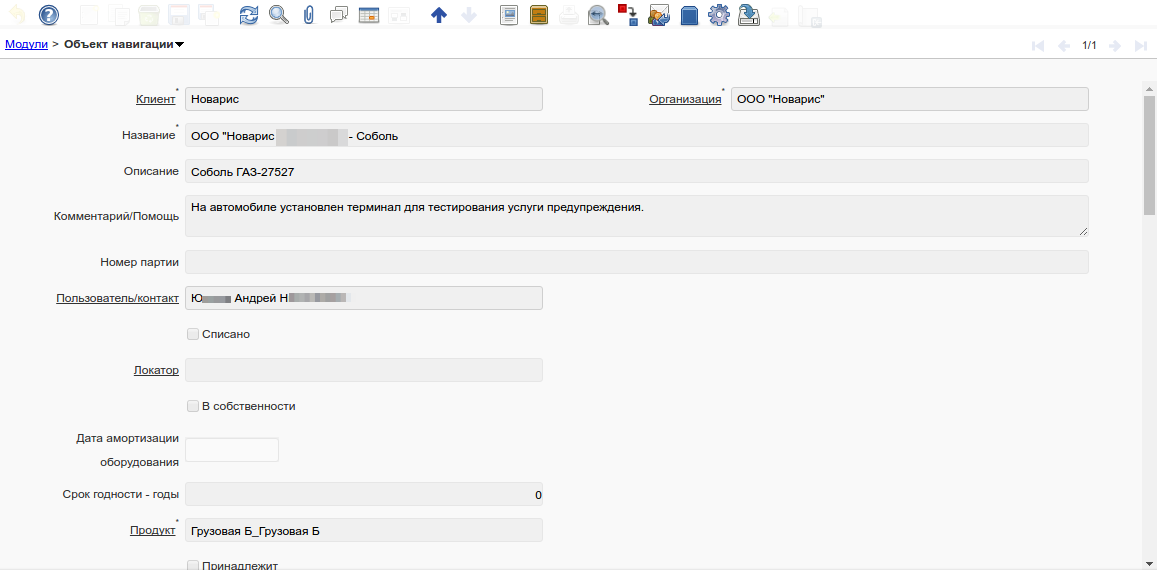
\includegraphics[width=0.9\linewidth]{mod01}}
  \end{center}
  \caption{Настройки клиентской машины.}
  \label{ris:imagemod01}
  \end{figure}
  
    \begin{figure}[h]
    \begin{center}
    \center{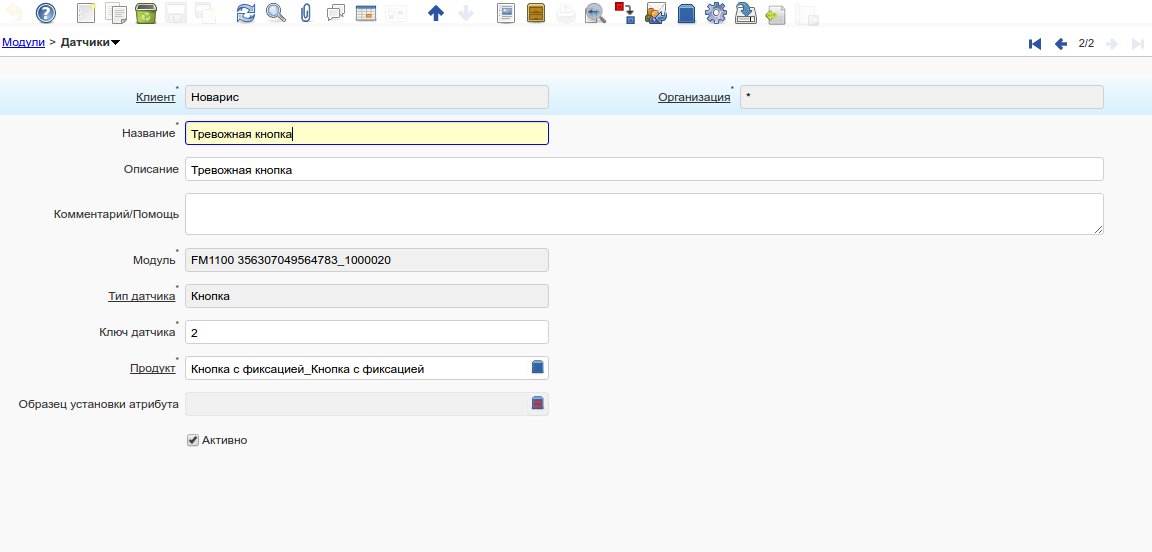
\includegraphics[width=0.9\linewidth]{mod02}}
    \end{center}
    \caption{Настройки датчика.}
    \label{ris:imagemod02}
    \end{figure}
    \begin{figure}[h]
    \begin{center}
    \center{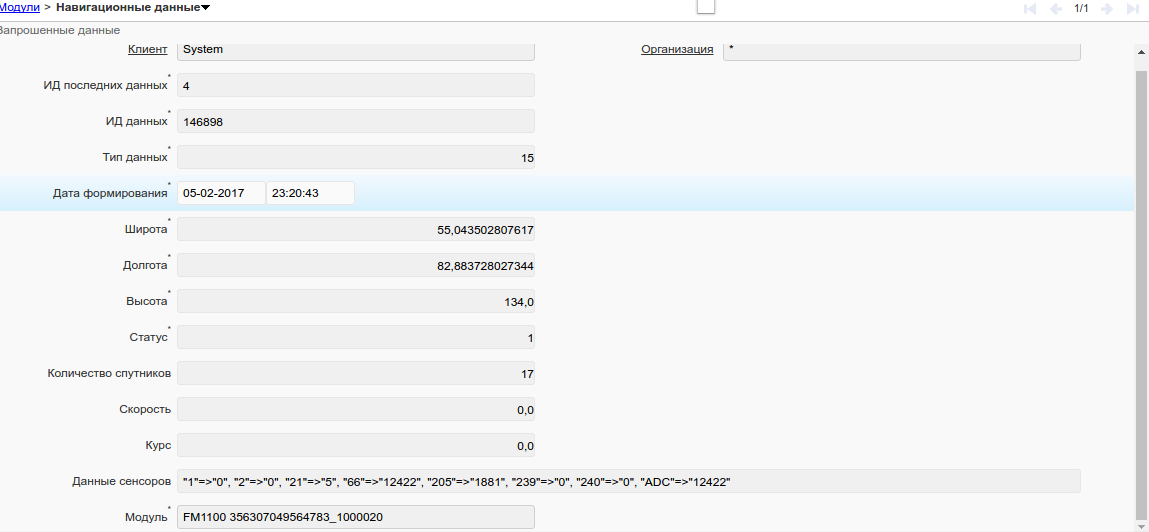
\includegraphics[width=0.9\linewidth]{mod03}}
    \end{center}
    \caption{Данные навигации.}
    \label{ris:imagemod03}
    \end{figure} 
\newpage
    
Выполнена настройка голосового помошника (IVR) для выбора услуги (записаны голосовые файлы, скрипт IVR подготовлен для обработки, настроен шаблон оповещения для вызова IVR). Выполнена привязка кода голосового меню к коду услуги системы Управления предприятием в конфиг файле.\label{begin01}

Выполнена настройка голосового помошника (IVR) для соединения Клиента и Водителя сервисной машины (записаны голосовые файлы, скрипт IVR подготовлен для обработки, настроен шаблон соединения для вызова IVR).\label{begin02}

Запущен сервис обработки услуг Системы управления предприятием.  
\newpage       
\subsection{Мониторинг}
\begin{longtable}[h]{|p{0.25\linewidth}|p{0.65\linewidth}|}
\hline
\textbf{Объект}& \textbf{Состояние}\\
\hline
Автомобиль клиента (Соболь XXX)& кнопка не нажата\\
\hline
Сервисный автомобиль поставщика услуги& кнопка не нажата\\
\hline
\end{longtable}
\subsection{Платформа}
Операторы платформы и услуги вошли в систему.
\begin{figure}[h]
\begin{minipage}[h]{0.9\linewidth}
\center{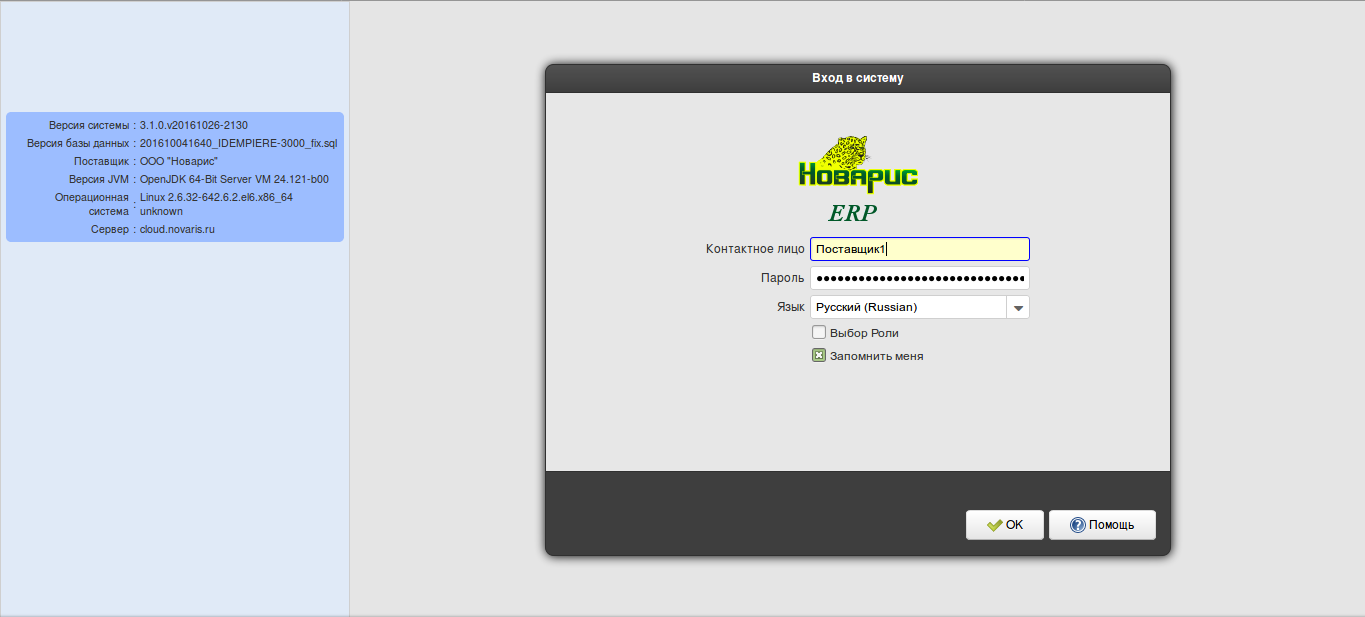
\includegraphics[width=0.9\linewidth]{01} \\ Вход Поставщика}
\end{minipage}
\hfill
\begin{minipage}[h]{0.9\linewidth}
\center{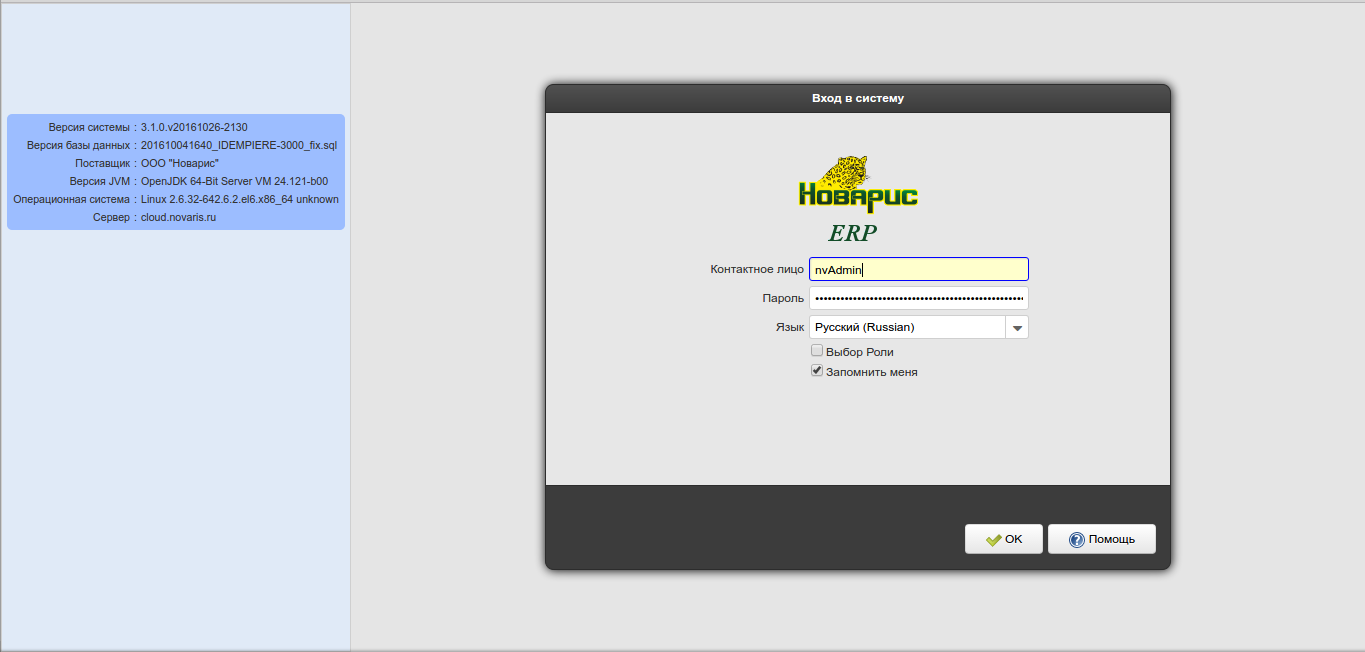
\includegraphics[width=0.9\linewidth]{02} \\  Вход Оператора}
\end{minipage}
\caption{Вход в систему.}
\label{ris:image1}
\end{figure}

\newpage
 \subsubsection{Поставщик услуги}
 Видит на карте только свою сервисную машину - иконка зелёная.
 \\
  Запросов на сервис "0".
  \begin{figure}[h]
  \begin{center}
  \center{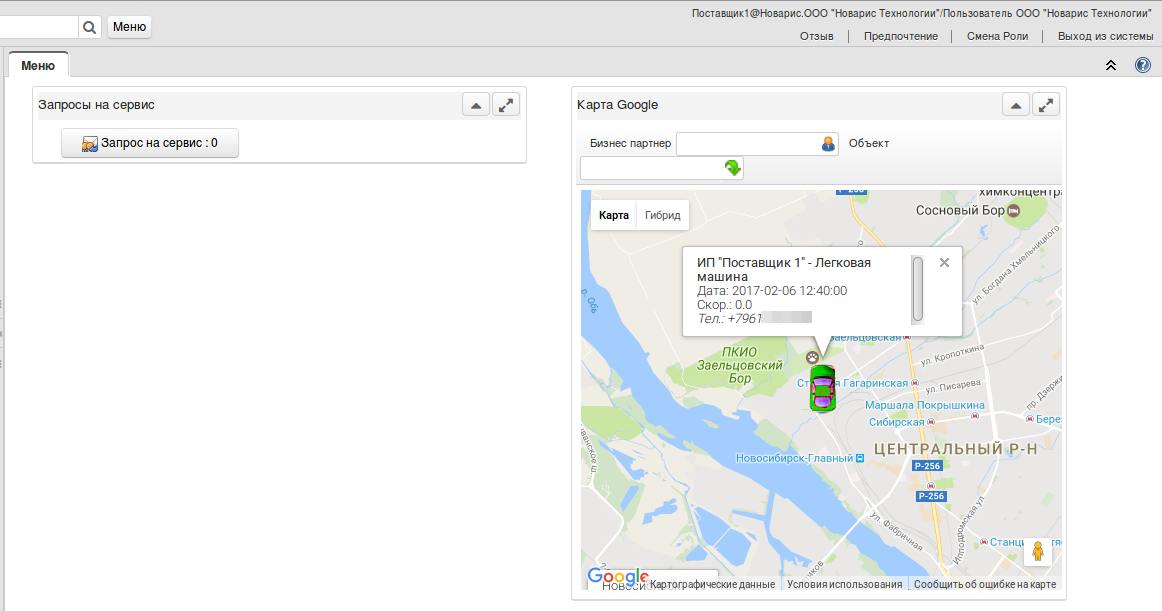
\includegraphics[width=0.9\linewidth]{03}}
  \end{center}
  \caption{Рабочая область Поставщика услуги.}
  \label{ris:image3}
  \end{figure}
 \newpage
 \subsubsection{Администратор платформы.} 
 Видит сервисную машину Поставщика услуги и машину Клиента - иконки зелёные.\\
 Запросов на сервис "0". 
\begin{figure}[h]
\begin{center}
\center{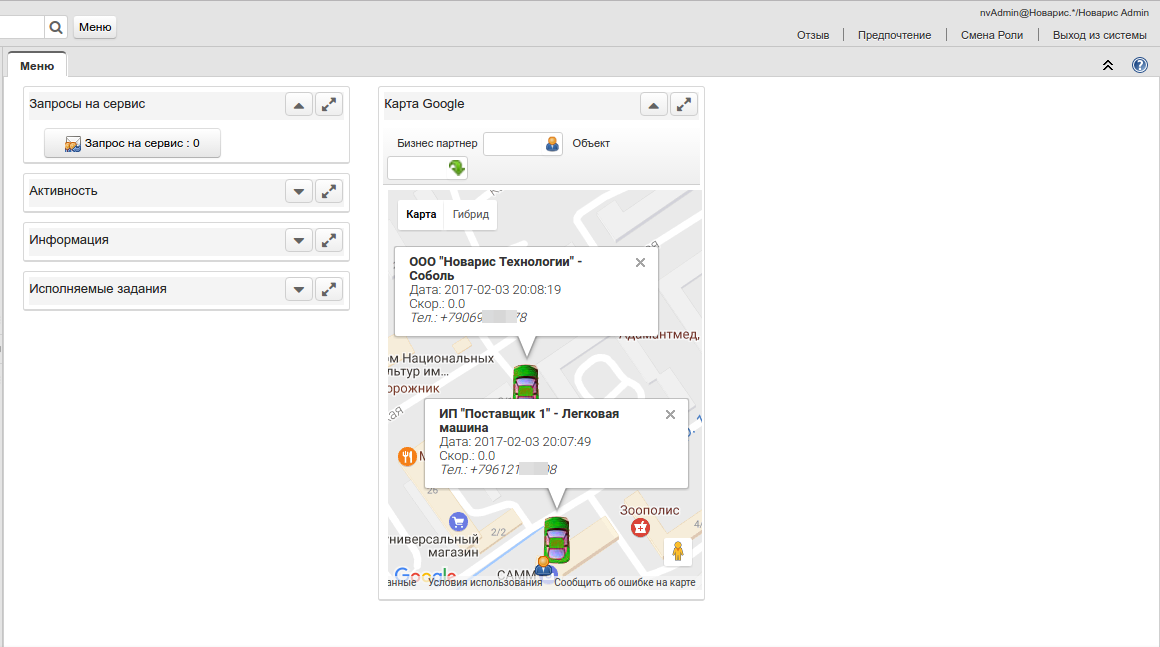
\includegraphics[width=0.9\linewidth]{04}}
\end{center}
\caption{Рабочая область Администратора платформы.}
\label{ris:image4}
\end{figure}

\section{Проведение тестирования}
\begin{enumerate}
\item На клиентской машине выполняется нажатие кнопки.
\item Терминал передаёт высоко приоритетное сообщение в систему мониторинга с задержкой до 5 сек.\label{event:01}

\item В момент передачи данных происходит:
\begin{enumerate}
\item в интерфейсе <<Администратора>> иконка клиентской машины изменяет цвет на красный и всплывает на карте информационное сообщение --- информация о номере и телефоне водителя. Время задержки возникновения события не более 1 минуты от события \ref{event:01};
\newpage
\begin{figure}[h]
\begin{center}
\center{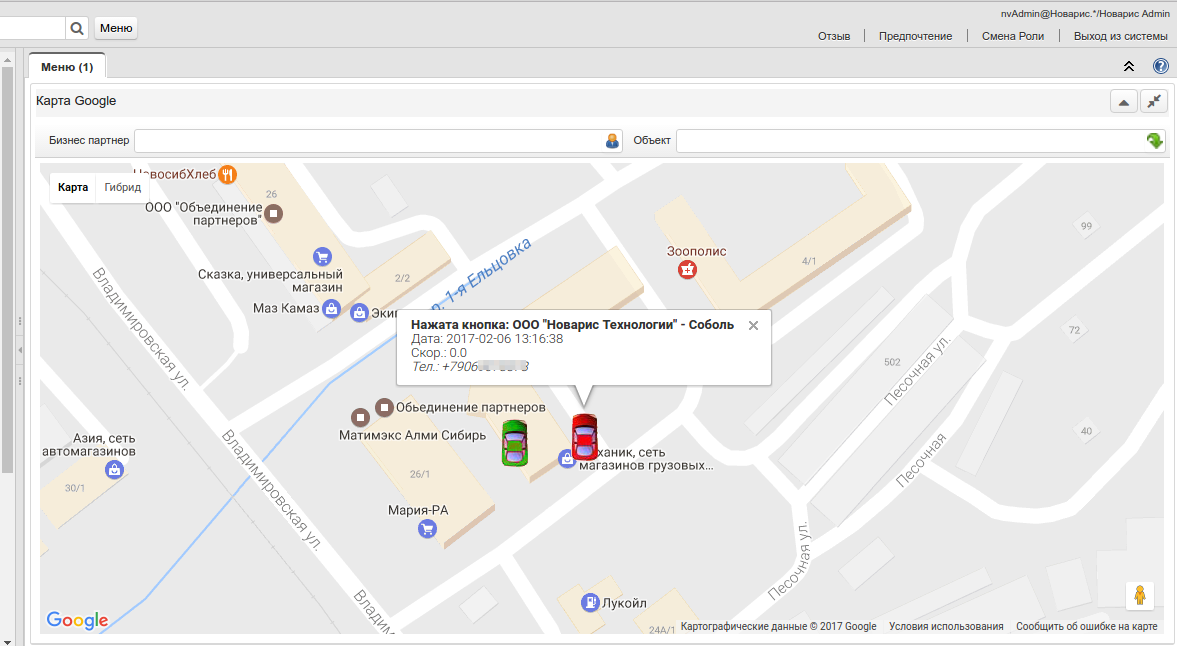
\includegraphics[width=0.9\linewidth]{05}}
\end{center}
\caption{Кнопка активирована на машине клиента.}
\label{ris:image5}
\begin{center}
\center{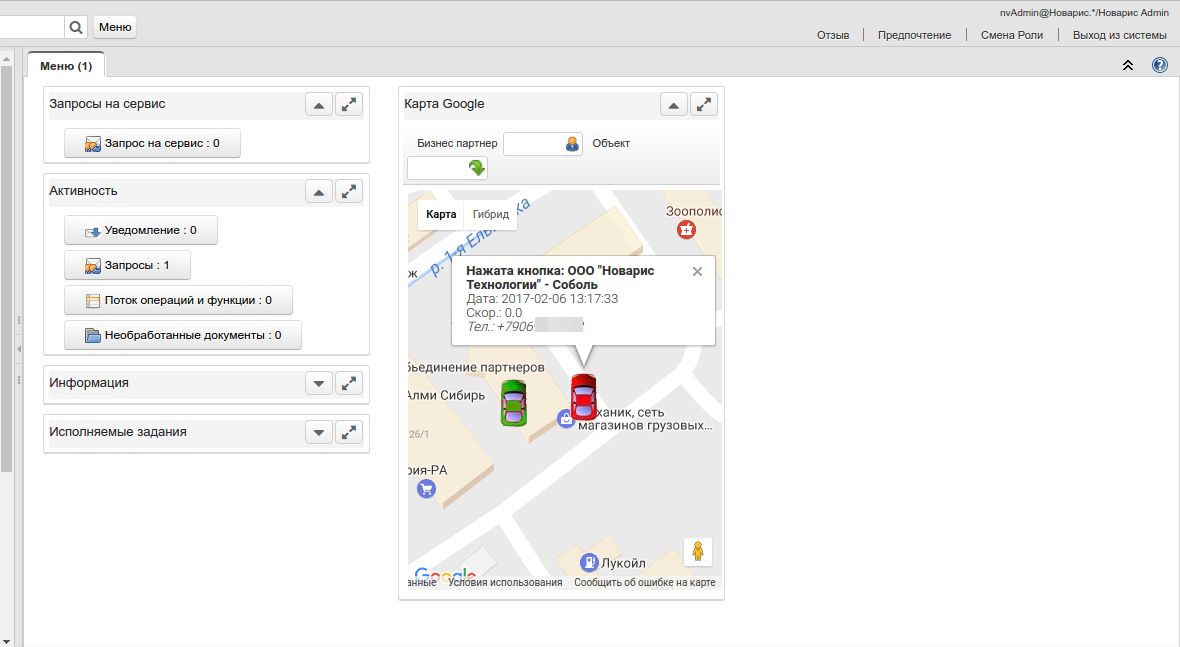
\includegraphics[width=0.9\linewidth]{06}}
\end{center}
\caption{Кнопка активирована на машине клиента.}
\label{ris:image6}
\end{figure};
\newpage
\item одновременно с получением события выполняется передача задания на обзвон на платформу обзвона с указанием типа шаблона обработки звонка, в данном случае это будет предварительно настроенный помощник с выбором услуги, задержка передачи задания не превышает 10 сек от события \ref{event:01}\label{event:02};
\begin{figure}[h]
\begin{center}
\center{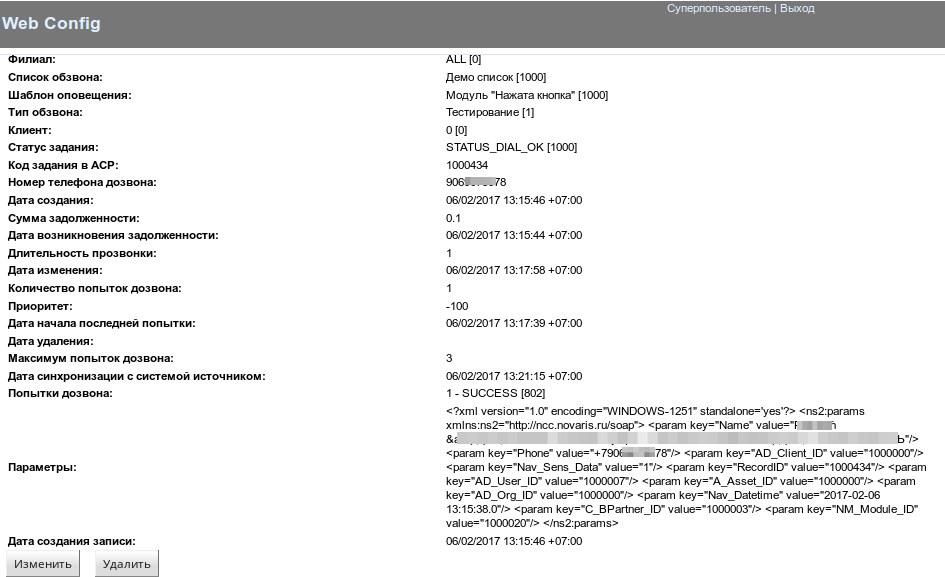
\includegraphics[width=0.9\linewidth]{ncs04}}
\center{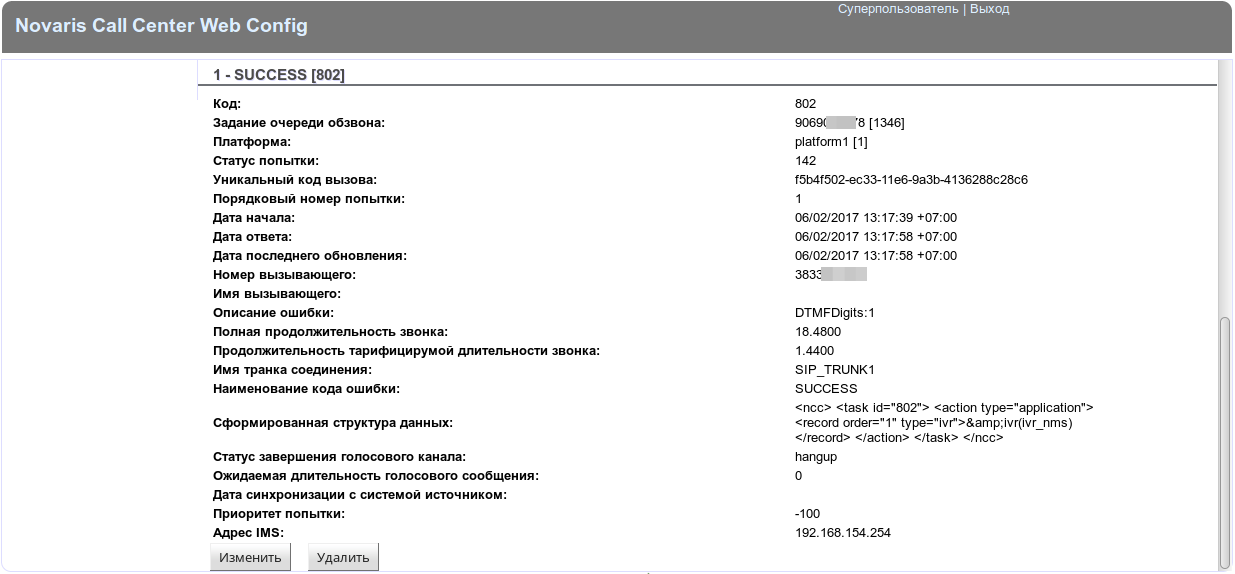
\includegraphics[width=0.9\linewidth]{ncs03}}
\end{center}
\caption{Выполнение задания на платформе обзвона}
\label{ris:image7}
\end{figure}


\item одновременно с изменением иконки, формируется в системе запись <<Запрос>> типа <<Запросы системы NCS>> в статусе 20 --- <<Обработка>> которая переходит в статус <<Обработка NCS>> при формировании задания на обзвон;
\item при любой операции с записью <<Запрос>> (создание записи или её изменение) выполняется отправка почты Администратору на указанный в его настройках e-mail;
\item запись <<Запрос>> содержит всю информацию необходимую для идентификации Клиента (ссылку на машин у с её атрибутами --- типом номером vin и т.п., телефон водителя нажавшего кнопку, ссылку на терминал с координатами и состоянием датчиков)
\end{enumerate}
\item Платформа обзвона по расписанию выполняет дозвон до клиента и предлагает выбрать услугу. Текущая настройка определяет максимальную задержку в 2 мин. от события \ref{event:01}.
\item Клиент с выбирает нужный пункт меню, данные сохраняются на платформе обзвона. Состояние обзвона можно увидеть через интерфейс системы обзвона взяв информацию о номере задания из данных запроса \ref{event:02}. Вид интерфейса:
\begin{figure}[h]
\begin{center}
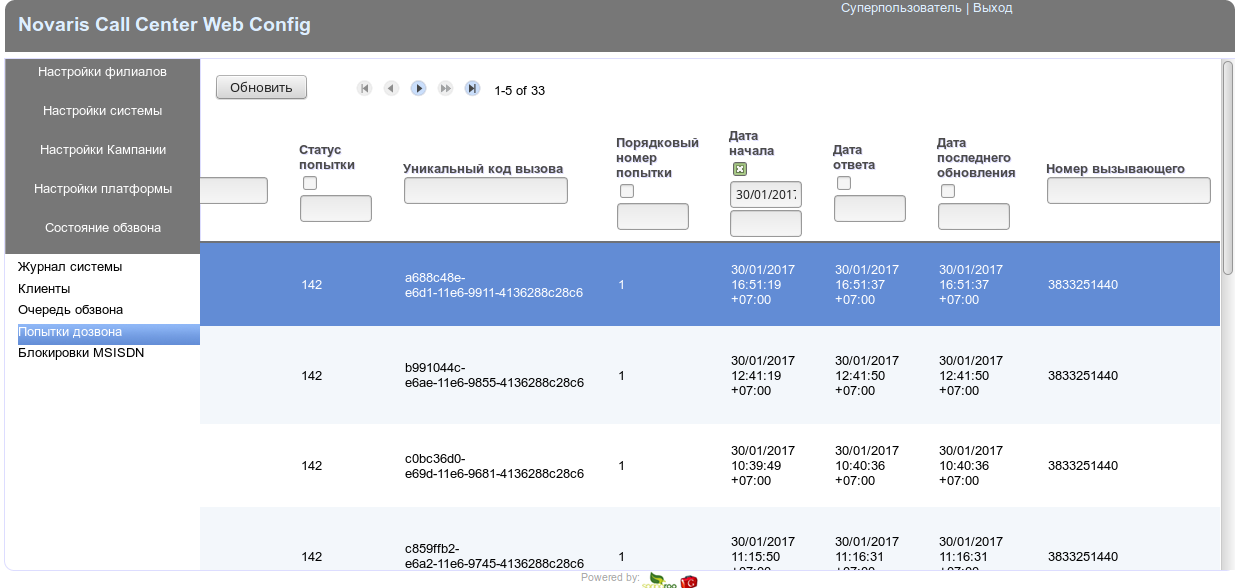
\includegraphics[width=0.9\linewidth]{ncs01}
\end{center}
\caption{Подсистема обзвона. Поиск попыток обзвона.}
\label{ris:ncs01}
\end{figure}
\begin{figure}[h]
\begin{center}
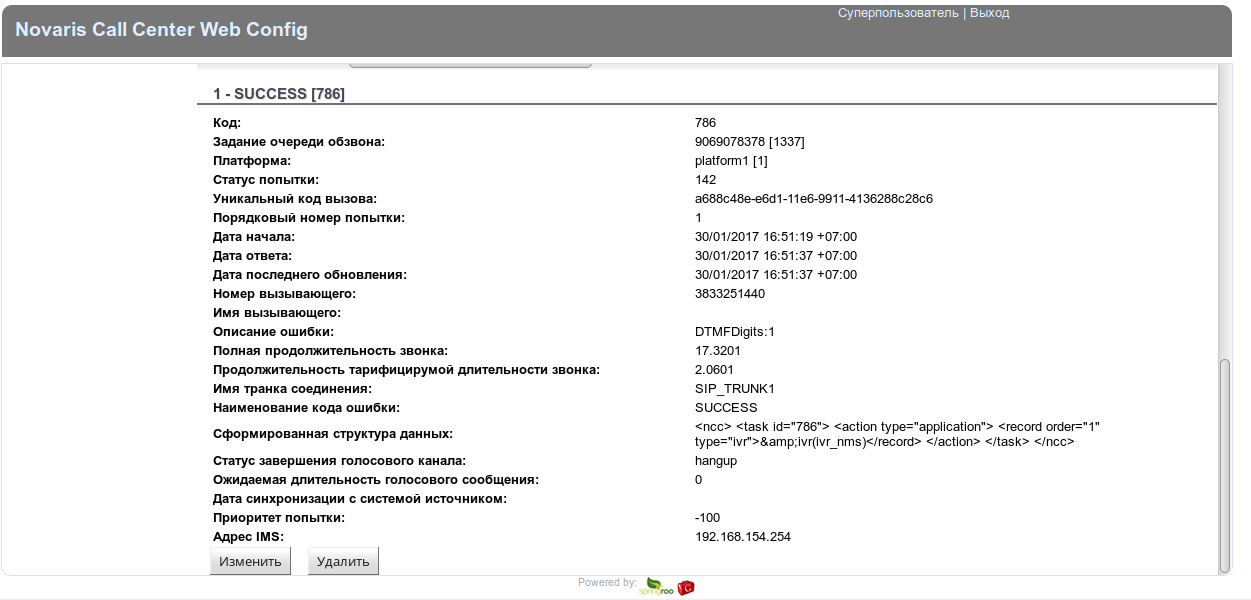
\includegraphics[width=0.9\linewidth]{ncs02}
\end{center}
\caption{Подсистема обзвона. Статус попытки обзвона.}
\label{ris:ncs02}
\end{figure}
\newpage
\item После выбора услуги Клиентом, система получает код код нажатой кнопки и сопоставляет с настроенной услугой в \ref{begin01}. Задержка от нажатия кнопки Клиентом до получения информации системой не превышает 10 сек.
\item После получения кода, процесс закрывает <<Запрос>> на выбор услуги, и открывает <<Запрос>> на предоставление выбранной услуги. Данный запрос отображается в интерфейсе Администратора. Дополнительно приходит e-mail. Параллельно с формированием запроса на услугу выполняются следующие действия (автоматически):
\begin{enumerate}
\item формируется запрос поставщикам;
\item выполняется поиск ближайшей свободной (кнопка --- свободен) машины (по прямой дистанции) и формируется выбор поставщика;
\item выбранному поставщику отсылается на электронную почту запрос на предоставления сервиса с параметрами (клиент, телефон и т.п.);
\item формируются бухг. документы (заказ на закупку у поставщика и заказ на продажу клиенту).
\item Выполняется звонок на сервисную машину Поставщика, после поднятия трубки водителем сервисной машины производится звонок на клиентскую машину. Выполняется разговор клиента и водителя сервисной машины поставщика с записью разговора на системе обзвона.   
\end{enumerate}
\item После автоматической привязки запроса клиента к поставщику --- поставщик увидит в своём интерфейсе клиентскую машину с отображением информации по телефону и дополнительной информации по водителю и машине (тип транспортного средства, ФИО водителя).
\newpage
\item В интерфейсе поставщика появляется запрос на сервис, по его нажатию открывается окно запроса на сервис, имеющее полную информацию по клиенту с расстоянием. Внизу формы доступен список свободных сервисных машин на которую может быть назначен, с указанием расстояния до них и в перспективе адресной информации.
\begin{figure}[h]
\begin{center}
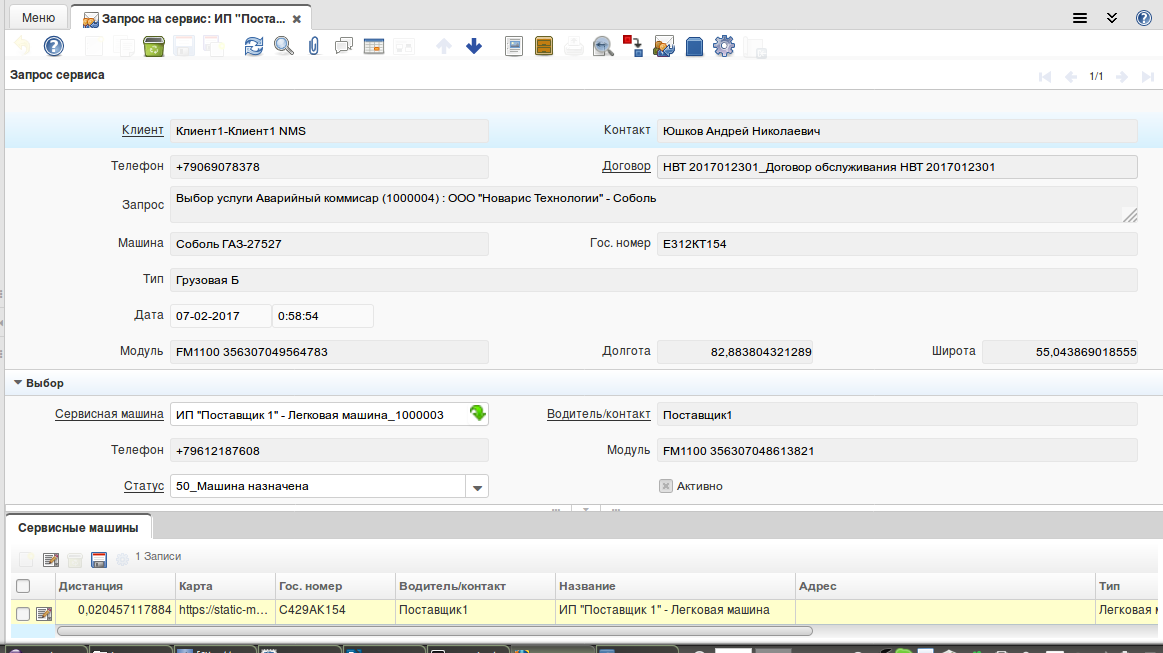
\includegraphics[width=0.9\linewidth]{09}
\end{center}
\caption{Окно состояния запроса на сервис.}
\label{ris:09}
\end{figure}
При нажатии на поле карта отобразится статичная информация о пробках и маршруте между клиентской и указанной сервисной машиной.
\begin{figure}[h]
\begin{center}
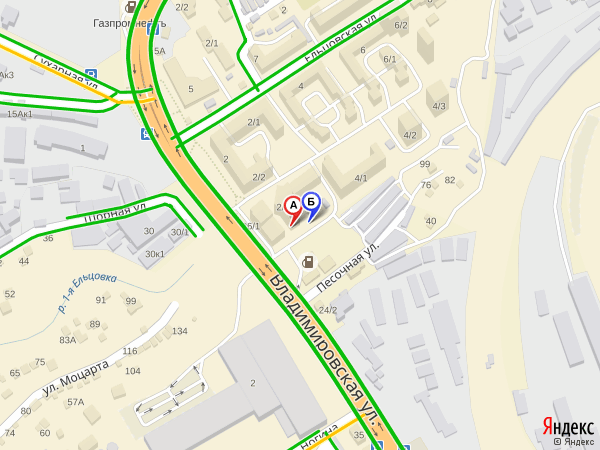
\includegraphics[width=0.5\linewidth]{10}
\end{center}
\caption{Окно информации о маршруте и пробках.}
\label{ris:10}
\end{figure}
\item Поставщик соглашается с выбором предложенным автоматом или выбирает другую сервисную машину и переводит Заявку на сервис в статус <<Машина назначена>>.
\item После завершения работ заявка переводится Поставщиком в статус завершение 
\end{enumerate}

\begin{appendix}
\section{Почтовые сообщение от системы для Администратора}
\begin{verbatim}
Обновил: nvAdmin
Создано: 2017-02-06 13:15:46.657
---------.----------.----------.----------.----------.----------
Запрос от объекта: Соболь XXX

---------.----------.----------.----------.----------.----------
Запросы: 1000417  [Req#1000434#ID]
Sent by iDempiereMail


Обновил: nvAdmin
Создано: 2017-02-06 13:15:46.657
Статус: 10_Инициация -> 30_Обработка NCS
---------.----------.----------.----------.----------.----------
Запрос от объекта: Соболь XXX
----------
Задание поставлено в очередь на обзвон. ИД задания NCS: 1346 [2017-02-06T13:15:46.000+07:00]

---------.----------.----------.----------.----------.----------
Запросы: 1000417  [Req#1000434#ID]
Sent by iDempiereMail


Обновил: nvAdmin
Дата последнего действия: 2017-02-06 13:15:46.657
Статус: 30_Обработка NCS -> 40_Обработана в NCS
---------.----------.----------.----------.----------.----------
Запрос от объекта: Соболь XXX
----------
Успешно обработано на платформе NCS: 1000

---------.----------.----------.----------.----------.----------
Запросы: 1000417  [Req#1000434#ID]
Sent by iDempiereMail



Обновил: nvAdmin
Создано: 2017-02-06 13:20:39.87
---------.----------.----------.----------.----------.----------
Выбор услуги Аварийный коммисар (1000004) : Соболь XXX

---------.----------.----------.----------.----------.----------
Запросы: 1000418  [Req#1000435#ID]
Sent by iDempiereMail



Обновил: nvAdmin
Создано: 2017-02-06 13:20:39.87
Статус: 10_Инициация -> 20_Обработка
---------.----------.----------.----------.----------.----------
Выбор услуги Аварийный коммисар (1000004) : Соболь XXX

---------.----------.----------.----------.----------.----------
Запросы: 1000418  [Req#1000435#ID]
Sent by iDempiereMail


Обновил: nvAdmin
Дата последнего действия: 2017-02-06 13:20:39.87
Статус: 20_Обработка -> 30_Обработка NCS
---------.----------.----------.----------.----------.----------
Выбор услуги Аварийный коммисар (1000004) : Соболь XXX
----------
Поставленое в очередь NCS: 1347 [2017-02-06T13:21:14.000+07:00]

---------.----------.----------.----------.----------.----------
Запросы: 1000418  [Req#1000435#ID]
Sent by iDempiereMail
\end{verbatim}
\section{Заявка на сервис при выборе поставщика}
\includepdf[pages=-]{ReportEngine.pdf}
\end{appendix}
\end{document}
